\documentclass[a4paper,11pt,twoside]{article}
%\documentclass[a4paper,11pt,twoside,se]{article}

\usepackage{UmUStudentReport}
\usepackage{verbatim}   % Multi-line comments using \begin{comment}
\usepackage{courier}    % Nicer fonts are used. (not necessary)
\usepackage{pslatex}    % Also nicer fonts. (not necessary)
\usepackage[pdftex]{graphicx}   % allows including pdf figures
\usepackage{listings}
\usepackage{pgf-umlcd}
\usepackage{blindtext}
\usepackage{enumitem}
\usepackage{amsfonts}
\usepackage{amssymb}
\usepackage{tikz}
\usetikzlibrary{shapes, positioning, calc}
\colorlet{lightgray}{gray!20}
%\usepackage{mathtools}

%\usepackage{lmodern}   % Optional fonts. (not necessary)
%\usepackage{tabularx}
%\usepackage{microtype} % Provides some typographic improvements over default settings
%\usepackage{placeins}  % For aligning images with \FloatBarrier
%\usepackage{booktabs}  % For nice-looking tables
%\usepackage{titlesec}  % More granular control of sections.

% DOCUMENT INFO
% =============
\department{Department of Computing Science}
\coursename{Introduction to Database Managment 7.5 p}
\coursecode{5DV119}
\title{Exercises, Chapter/Topic 4}
\author{Lorenz Gerber ({\tt{dv15lgr@cs.umu.se}} {\tt{lozger03@student.umu.se}})}
\date{2017-02-21}
%\revisiondate{2016-01-18}
\instructor{Jan Erik Moström / Michael Minock / Filip Allberg / Carl-Anton Anserud}


% DOCUMENT SETTINGS
% =================
\bibliographystyle{plain}
%\bibliographystyle{ieee}
\pagestyle{fancy}
\raggedbottom
\setcounter{secnumdepth}{2}
\setcounter{tocdepth}{2}
%\graphicspath{{images/}}   %Path for images

\usepackage{float}
\floatstyle{ruled}
\newfloat{listing}{thp}{lop}
\floatname{listing}{Listing}



% DEFINES
% =======
%\newcommand{\mycommand}{<latex code>}
%\DeclarePairedDelimiter{\ceil}{\lceil}{\rceil}

% DOCUMENT
% ========
\begin{document}
\lstset{language=C}
\maketitle
\thispagestyle{empty}
%\newpage
%\tableofcontents
\thispagestyle{empty}
\newpage

\clearpage
\pagenumbering{arabic}

\section{Introduction}

\section{Mapping Step by Step}

\section{Final Results}

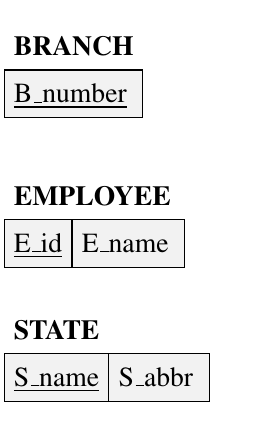
\begin{tikzpicture}[relation/.style={rectangle split,
      rectangle split parts=#1,
      rectangle split part align=base,
      draw,
      anchor=center,
      align=center,
      text height=3mm,
      text centered}]
  \hspace*{-0.3cm}

  % RELATIONS

  \node (branchtitle) {\textbf{BRANCH}};

  \node[relation=1,
    rectangle split horizontal,
    rectangle split part fill={lightgray!50},
    anchor=north west,
    below=0.6cm of branchtitle.west,
    anchor=west](branch) {
    \underline{B\_number}
  };

  \node [below=1.3cm of branch.west,
    anchor=west] (employeetitle) {
    \textbf{EMPLOYEE}
  };


  \node [relation=2,
    rectangle split horizontal,
    rectangle split part fill={lightgray!50},
    below=0.6cm of employeetitle.west,
    anchor=west] (employee) {
    \underline{E\_id}%
    \nodepart{two} E\_name
  };

  \node [below=1.1cm of employee.west,
    anchor=west] (statetitle) {
    \textbf{STATE}
  };


  \node [relation=2,
    rectangle split horizontal,
    rectangle split part fill={lightgray!50},
    anchor=north west,
    below=0.6cm of statetitle.west,
    anchor=west] (state) {
    \underline{S\_name}%
    \nodepart{two}   S\_abbr
  };

\end{tikzpicture}



\addcontentsline{toc}{section}{\refname}
%\bibliography{references}

\end{document}
